% !TeX root = Thesis.tex

\chapter{Related~Works}
\label{chap:related_works}

In this chapter, we review prior works on two topics related to our research: \nameref{sec:3d_representations}s and \nameref{sec:representation_learning_architectures}.

\section{3D~Representations}
\label{sec:3d_representations}

There are a multitude of methods for digitally representing a 3D volume. Any representation can be used in machine learning, but each has different benefits and challenges. In this section, we discuss the five most common 3D representations in the literature and their applications in machine learning.


\subsection{Point~Cloud}
\label{subsec:point_cloud}

\begin{figure}[h]
	\centering
	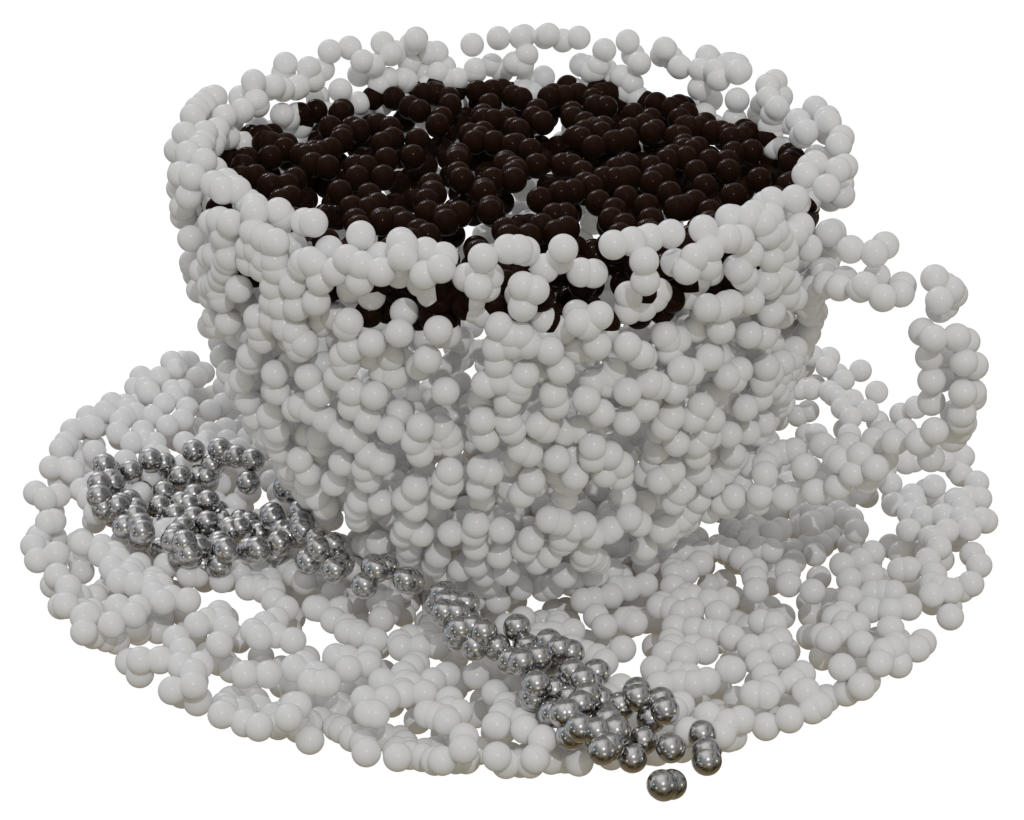
\includegraphics[scale=0.2]{Images/Point Cloud Cup}
	\caption{Point cloud representation of a coffee cup.}
	\label{fig:point_cloud_cup}
\end{figure}

A point cloud is set of unordered 3D coordinates sampled from an object's surface. Point clouds are unstructured and lack topological data~\cite{Xiao2020}. However, this simplicity makes it easy to acquire point clouds using 3D scanning technologies such as lidar and photogrammetry~\cite{Leberl2010}. Photogrammetry is an algorithm that uses multiple photos taken from different angles to triangulate points on a surface. A photogrammetry scan can be performed with even a smartphone, greatly increasing the accessibility of point cloud scans~\cite{Micheletti2015}.

Despite its accessibility, point clouds didn't see use in 3D learning techniques until 2017~\cite{Xiao2020}. The seminal work PointNet~\cite{Qi2017} used a Multi-Level Perceptron (MLP) encoder to demonstrate that point clouds can be processed directly to solve problems such as classification and part segmentation. The follow up work PointConv~\cite{Wu2019} saw similar success using a Convolutional Neural Network (CNN) encoder. Further works~\cite{Fan2017, Achlioptas2018} have demonstrated that deep learning models can be trained to reconstruct an input as a point cloud. Although point clouds only offer a sparse approximation of a surface, their low-dimensionality proves useful in efficiently learning 3D features.


\subsection{Polygon~Mesh}
\label{subsec:polygon_mesh}

\begin{figure}[h]
	\centering
	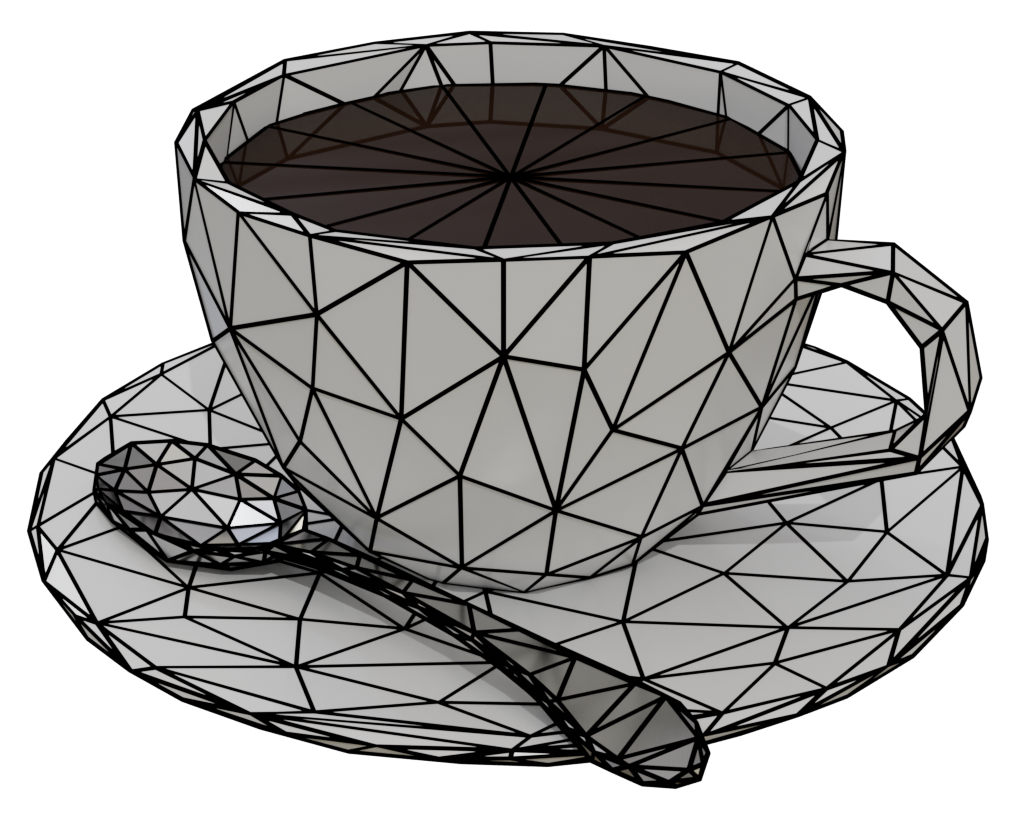
\includegraphics[scale=0.2]{Images/Mesh Cup}
	\caption{Triangle mesh representation of a coffee cup. The black lines depict the connecting edges between vertices.}
	\label{fig:mesh_cup}
\end{figure}

Mesh-based models consist of vertices connected by flat polygonal faces. Unlike point clouds, meshes can represent topology and surface details~\cite{Xiao2020}. Polygon meshes are the most popular 3D representation for use in computer graphics since they are easy to render into images~\cite{Watt1996}. Another unique benefit is that meshes are easy to deform and animate~\cite{Wang2018}. These qualities make mesh-based models ideal for use in video games, virtual reality, and film~\cite{Nash2020}. One issue is that mesh models cannot be directly acquired using 3D scanners. This is easily circumvented, however, by using surface reconstruction techniques to generate high-quality mesh models from point cloud scans~\cite{Yuan2022}.

The prevalence of polygon meshes has motivated many mesh-based deep learning models. Since the structure of a polygon mesh is complex, these models adopt unique architectures to simplify the problem. To directly process polygon meshes, models such as FeaStNet~\cite{Verma2018} and MeshCNN~\cite{Hanocka2019} employ Graph Convolutional Networks (GCN). A mesh can be seen as a directed graph of interconnected nodes. This enables graph-based methods such as GCN to directly consume meshes as input. While a traditional CNN applies filters to a group of pixels in an image, a GCN applies filters to a group of nodes or edges in a graph. Like CNNs, GCNs support pooling operations to extract features from a mesh~\cite{Verma2018}. In addition to pooling operations, MeshCNN introduces graph-based unpooling operations to increase the resolution of a mesh.

Techniques to generate meshes are more varied. AtlasNet~\cite{Groueix2018} uses MLPs to reconstruct a point cloud out of 2D meshes. The model starts with a flat planes  as a template. The planes are then deformed to represent the surface of the point cloud. At the end, all the planes are stitched together. This papier-m\^{a}ch\'{e} approach is efficient but does not produce a continuous surface~\cite{Groueix2018}. Pixel2Mesh~\cite{Wang2018} and Point2Mesh~\cite{Hanocka2020} both deform a 3D template mesh through cascaded refinement to represent the input. Instead of a flat plane, Pixel2Mesh and Point2Mesh start with a sphere encompassing a point cloud. The template is then deformed in a coarse-to-fine manner with the resolution of the template mesh increasing each iteration. Starting with a lower resolution allows the model to quickly build a rough approximation of the shape. Then the resolution is gradually increased to allow for more fine adjustments as needed. Working with the minimum required resolution for any given iteration greatly improves the efficiency of these models. Unlike AtlasNet, Pixel2Mesh and Point2Mesh are guaranteed to generate continuous and manifold surfaces since the initial template shape is manifold. A limitation of current deformation based works is that they can only reconstruct genus 0 shapes. The models have no means to merge or remove geometry to represent holes~\cite{Wang2018, Hanocka2020}.

PolyGen~\cite{Nash2020} takes the most direct approach in generating 3D meshs. A vertex generation network predicts a variable number of vertices to represent the input. Then the vertices are fed to a face generation network that generates faces to best connect the vertices. Both networks are implemented as transformers, which process sequential data but generate the entire output at once. Transformers have a fixed output size, so the authors added a stopping token to the outputs of the vertex network to allow for variable size meshes. The maximum resolution of model was set to 1200 vertices 800 faces. Because Polygen directly generates meshes, it can represent geometric shapes with far fewer polygons than related works. The biggest limitation of PolyGen is its small output resolution. The computational cost of a transformer network increases quadratically with the size of the network. Despite some optimizations, the transformer networks are too inefficient at scale to generate more detailed meshes. Due to this limitation, PolyGen is focused on representing simple geometric shapes with the minimum number of polygons~\cite{Nash2020}.


\subsection{Occupancy~Grid}
\label{subsec:occupancy_grid}

\begin{figure}[h]
	\centering
	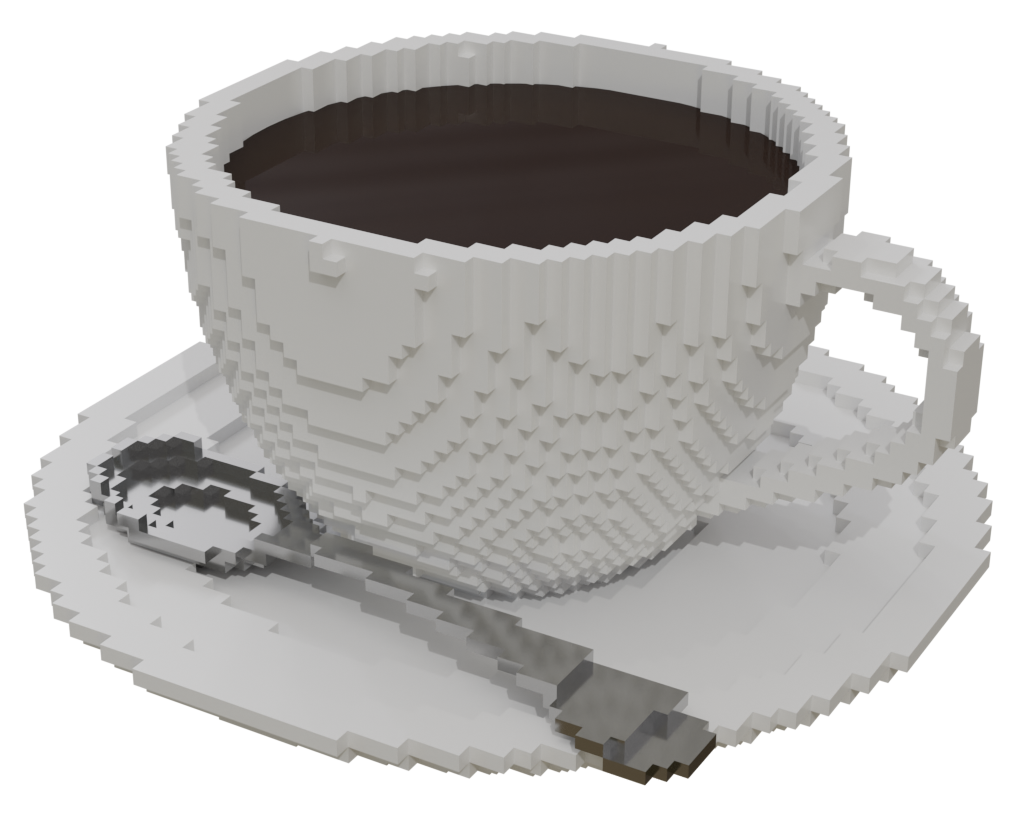
\includegraphics[scale=0.2]{Images/Voxel Cup}
	\caption{Voxel grid representation of a coffee cup.}
	\label{fig:voxel_cup}
\end{figure}

\subsection{Images}

\begin{figure}[h]
	\centering
	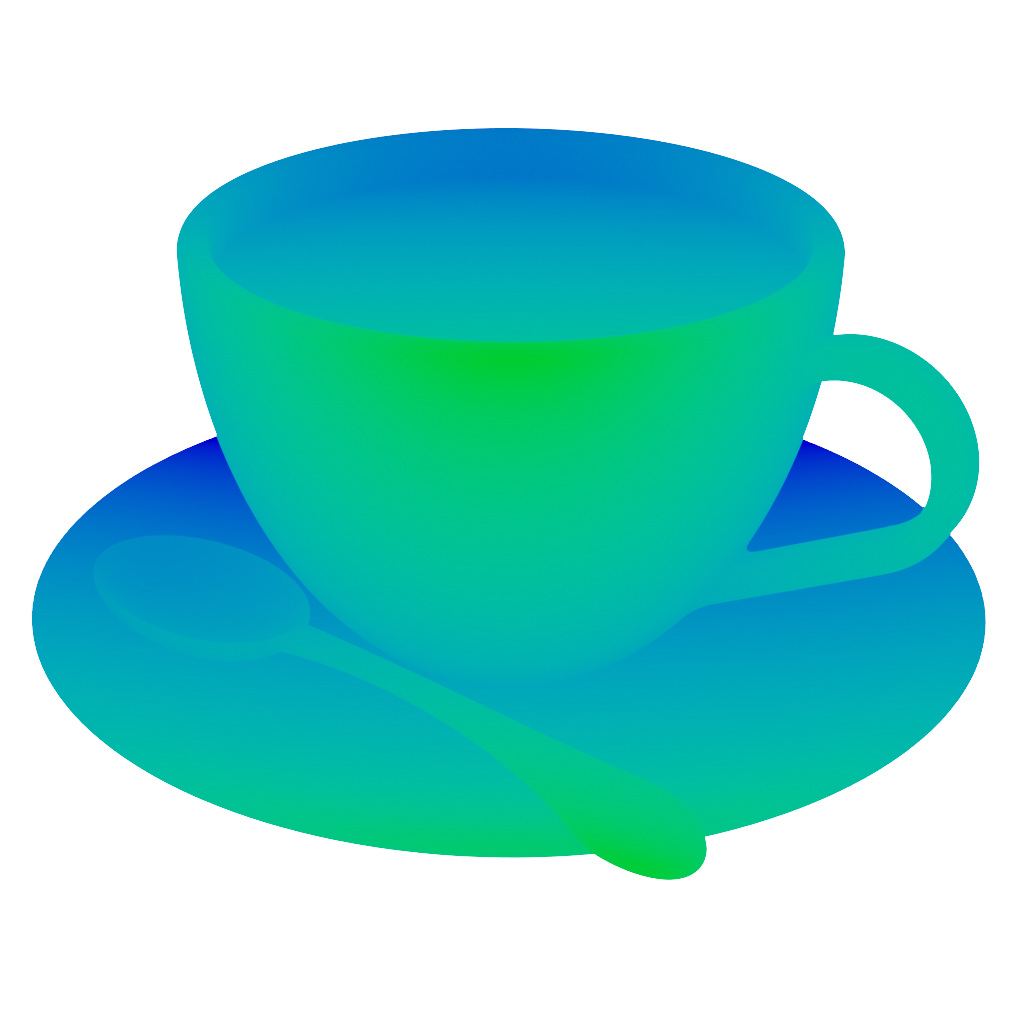
\includegraphics[scale=0.2]{Images/Depth Map Cup}
	\caption{Depth map representation of a coffee cup.}
	\label{fig:depth_map_cup}
\end{figure}

\subsection{Implicit~Surface}
\label{subsec:implicit_surface}

\begin{figure}[h]
	\centering
	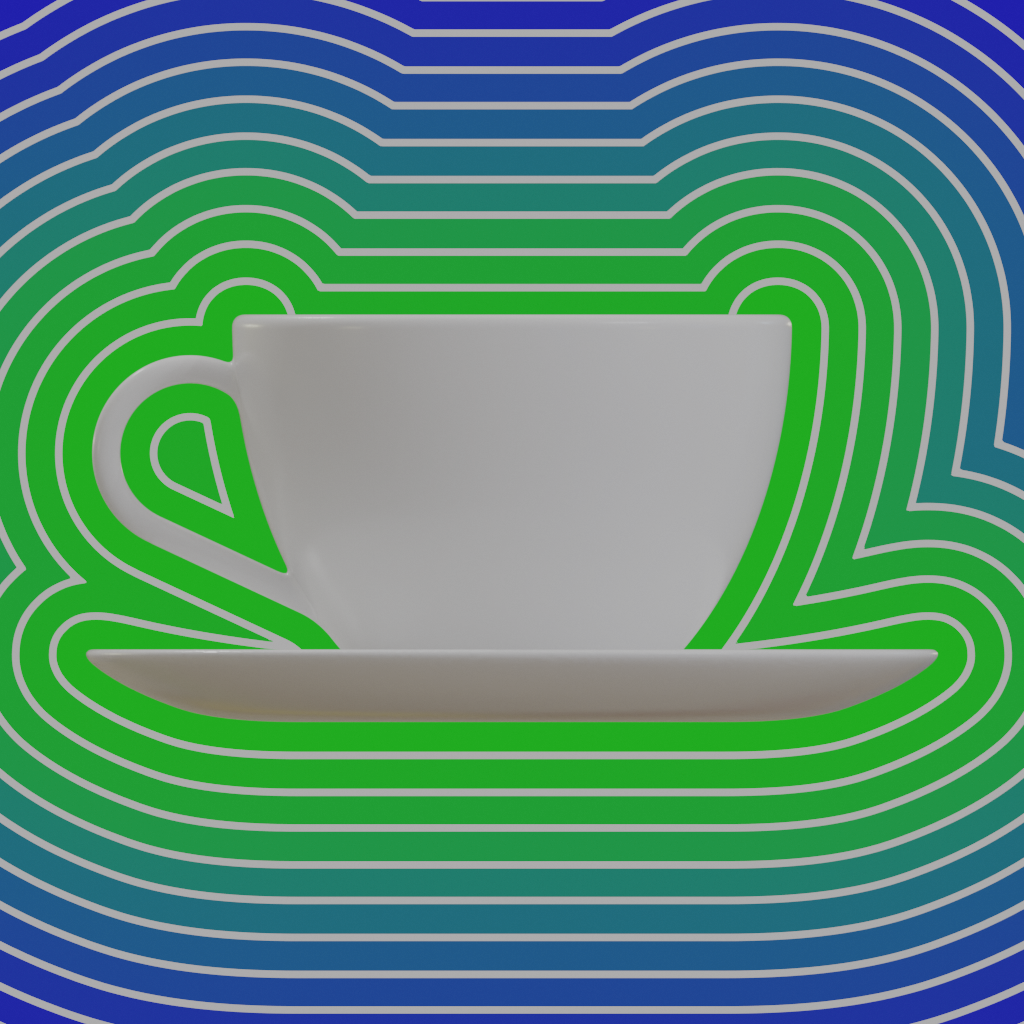
\includegraphics[scale=0.2]{Images/SDF Cup}
	\caption{Visualization of an SDF representing a coffee cup. Points close to the surface are drawn green and points far from the surface are drawn blue. Each white contour line consists of points that are equidistant from the surface.}
	\label{fig:sdf_cup}
\end{figure}

\subsection{Structured~Representation}
\label{subsec:structured_representation}

\begin{figure}[h]
	\centering
	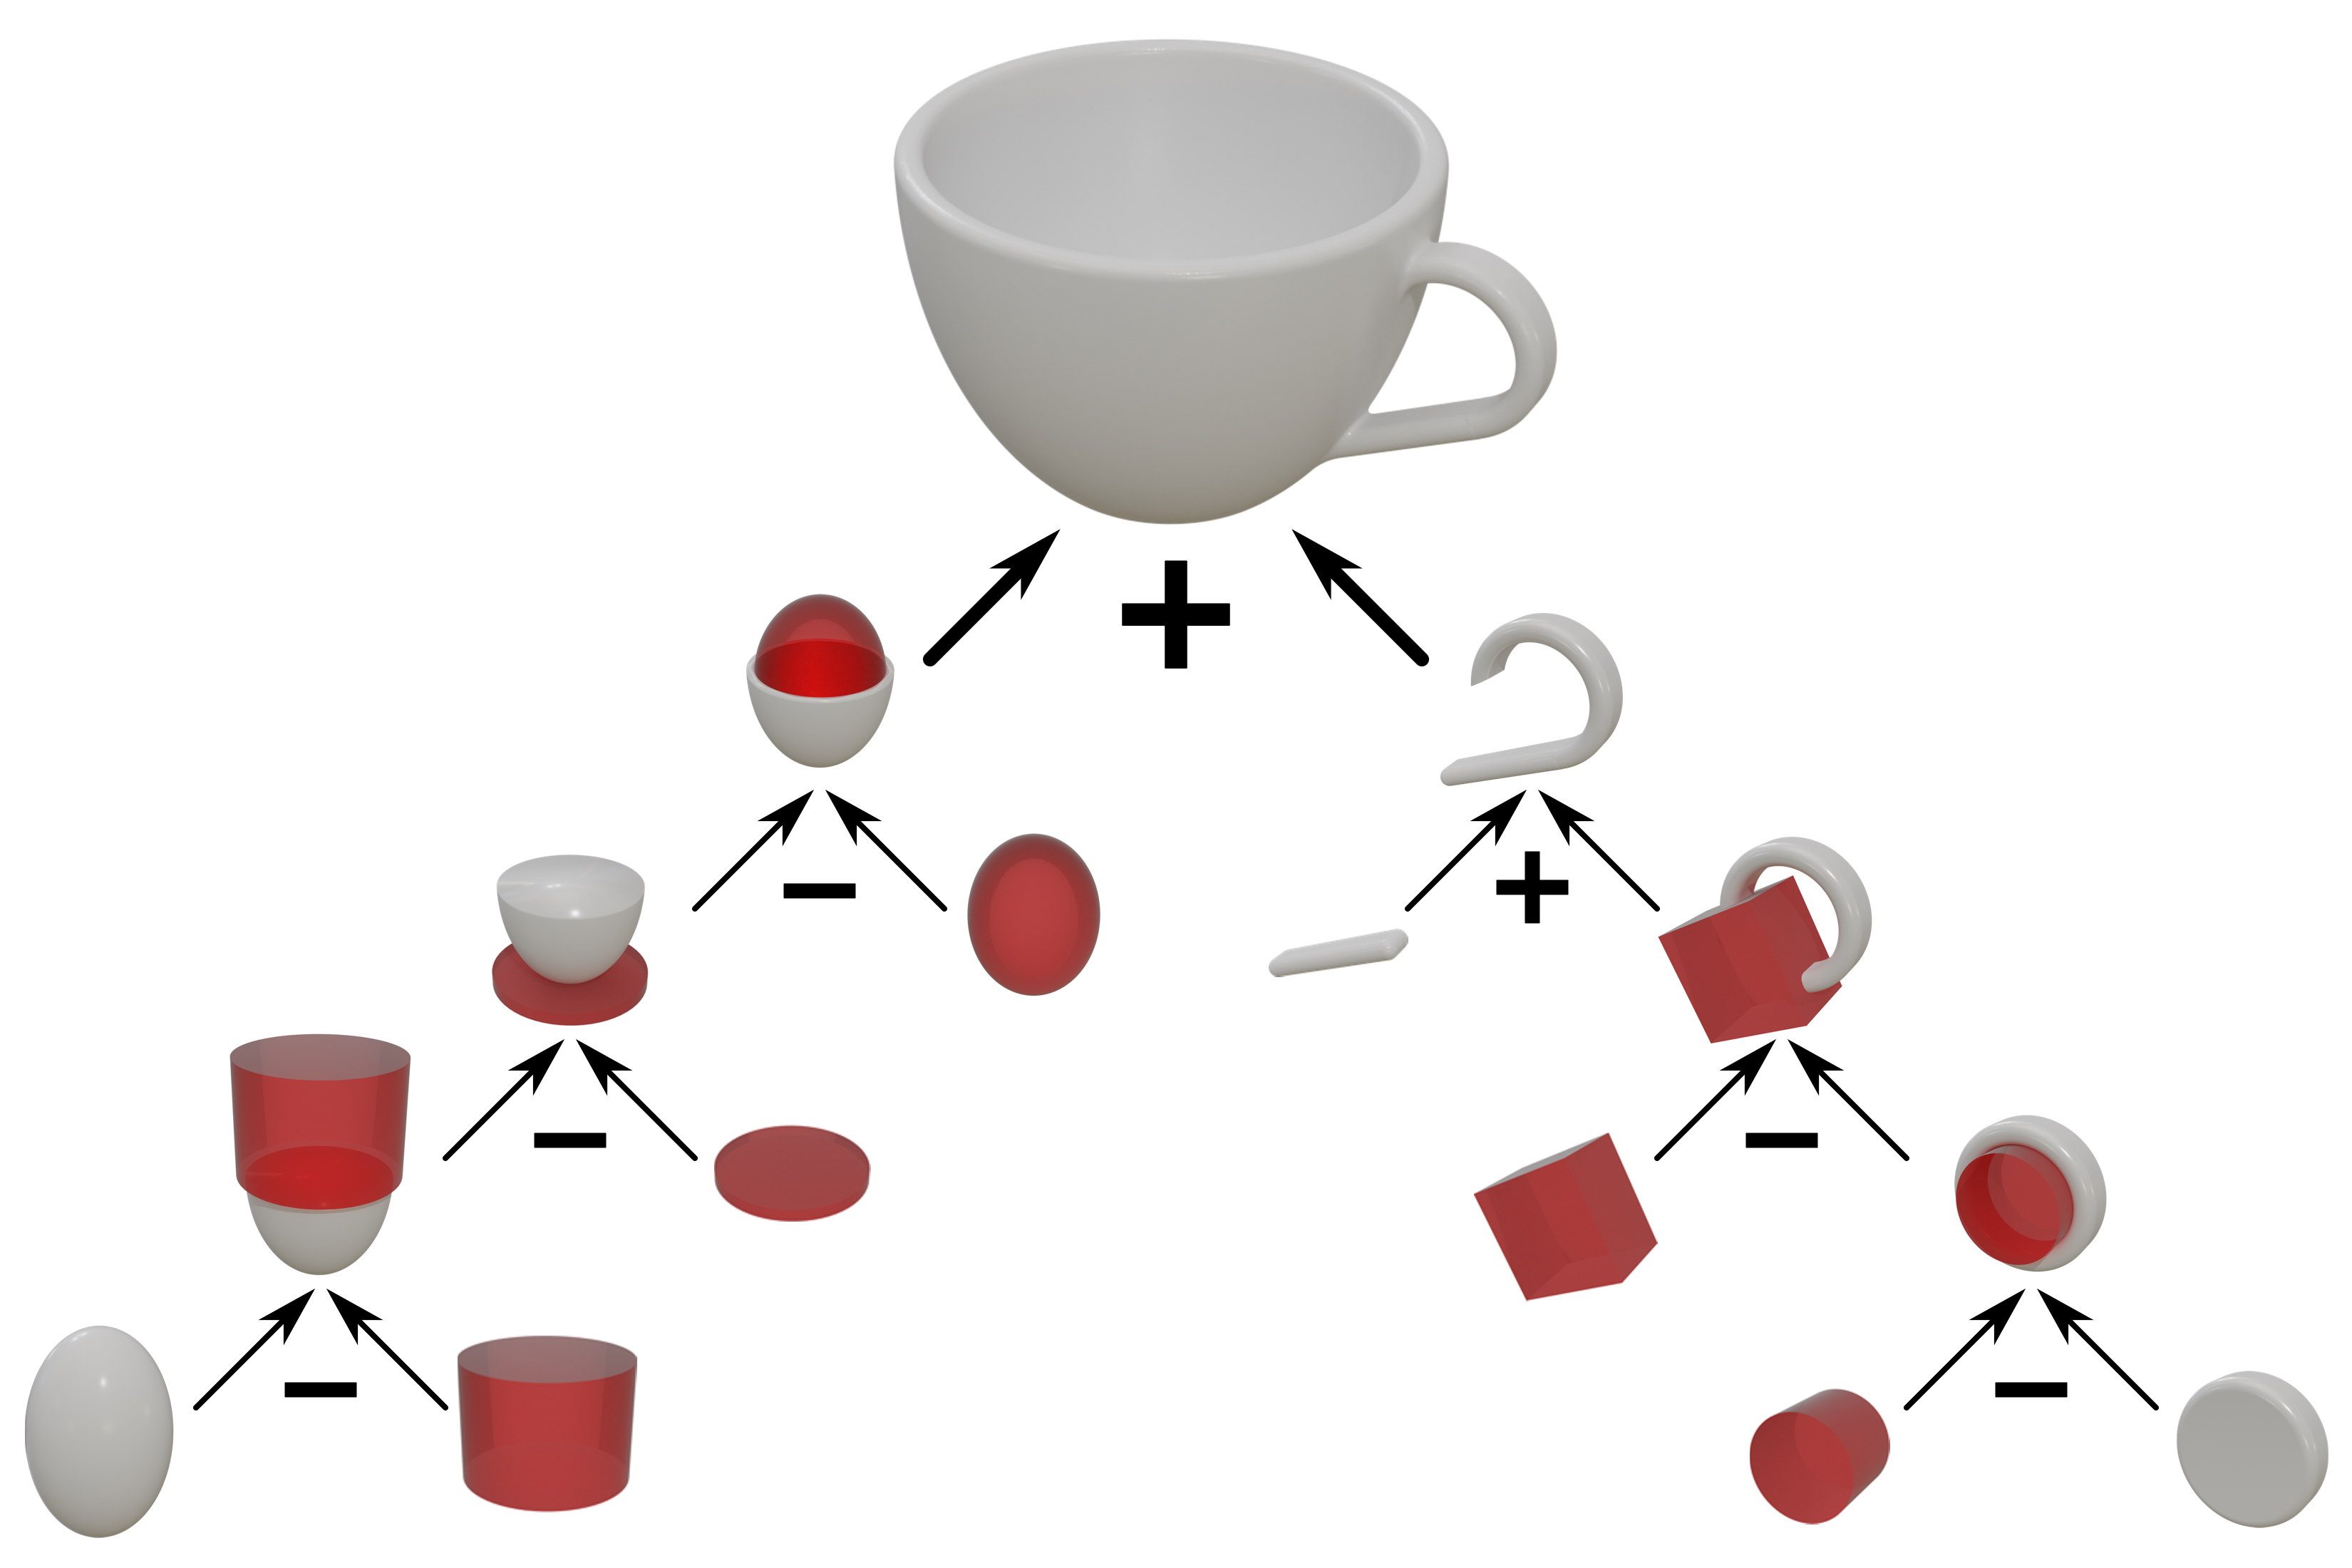
\includegraphics[scale=0.5]{Images/CSG Cup}
	\caption{The CSG tree of a coffee cup. The leaves of the tree are SDF primitives which are combined through union (+) and difference (-) operations. The primitives being subtracted are colored red.}
	\label{fig:csg_cup}
\end{figure}


\section{Representation~Learning~Architectures}
\label{sec:representation_learning_architectures}

Test

\subsection{Generative~Adversarial~Network}
\label{subsec:generative_adversarial_networks}

Test

\subsection{Autoencoder}
\label{subsec:autoencoders}

Test

\subsection{Cascaded~Refinement}
\label{subsec:cascaded_refinement}

Test